\definecolor{exxetagray}{gray}{0.75}
\definecolor{itemcolor}{RGB}{179,217,255}
\definecolor{usercolor}{RGB}{255,204,179}

\shorthandoff{"}
\chapter{Ergebnisse}
\label{ch:ergebnisse}

\section{Überblick Befragung der Mitarbeitenden}
An der Befragung der Mitarbeitenden bei EXXETA nahmen 54 Mitarbeitende aus insgesamt neun verschiedenen Teams teil.
Der Großteil der Befragten ($\approx$ 70 Prozent) stellten Mitarbeitende aus dem Team Java Enterprise Solutions dar, wobei sich die übrigen Mitarbeitenden nahezu gleichmäßg auf die anderen acht Teams (Business Application Development???) verteilt.
Die Befragung war für Mitarbeitende jedes Senioritätsniveaus und jeder Stellenbeschreibung zugängig.

% Von den 31 angefragten Fähigkeiten gaben Mitarbeitende im Mittel bei 38 Prozent der Fähigkeiten an Grundkenntnisse und bei 19 Prozent fortgeschrittene Kenntnisse zu besitzen (Werte aufgerundet auf die 2. Nachkommastelle).
% Bei knapp 43 Prozent der Fähigkeiten gaben die Befragten an, keine Kenntnisse zu besitzen.
% Von den angefragten Fähigkeiten wurden die Fähigkeiten "Backend" und "Git" von den meisten Mitarbeitenden beherrscht, während die Fähigkeit "Camunda" von den wenigsten Befragten besessen wurde.

% Von den angefragten Fähigkeiten wollten die befragten Mitarbeitenden im Durchschnitt 42 Prozent der Fähigkeiten in zukünftigen Projekten (weiter) anwenden.
% Bei 22 Prozent der Fähigkeiten gaben Mitarbeitende an, die Fähigkeit zukünftig (vorerst) nicht (weiter) anwenden zu wollen.
% Für 36 Prozent der Fähigkeiten gaben die Befragten an, der Möglichkeit, die Fähigkeit in zukünftigen Projekten anzuwenden, neutral gegenüber zu stehen.
% Übergreifend wurde die Fähigkeit "Git" von den meisten Mitarbeitenden präferiert, während die Fähigkeit "\ac{SOAP}" von den wenigsten Mitarbeitenden präferiert wurde.
% Der Fähigkeit "Helm" standen die meisten Mitarbeiter neutral gegenüber.
Insgesamt gaben die Befragten bei 960 der möglichen 1.674 Fähigkeiten (54 Probanden \`{a} je 31 Fähigkeitsbewertungen) an, diese zu beherrschen, während sie bei den übrigen 714 Fähigkeiten angaben, keine Kenntnisse zu besitzen.
Von den beherrschten Fähigkeiten gaben die Mitarbeitenden bei zwei Drittel der Fähigkeiten an über Grundkenntnisse und bei den restlichen ein Drittel über fortgeschrittene Kenntnisse zu verfügen.
Bezüglich der Präferenzen gaben die Befragten bei einem Großteil (696 Bewertungen) der zu bewertenden Fähigkeiten an, diese zukünftig (weiter) in Projekten anwenden zu wollen.
Bei ähnlich vielen Fähigkeiten (607 Bewertungen) gaben die Mitarbeitende an, der Option, die Fähigkeit in zukünftigen Projekten anzuwenden, neutral gegenüberzustehen.
Lediglich bei rund einem Fünftel der bewerteten Fähigkeiten gaben die Befragten an, die Fähigkeit zukünftig (vorerst) nicht (weiter) anwenden zu wollen.

Die durchschnittliche Verteilung der Fähigkeiten und Präferenzen je Mitarbeitendem ist in Abbildung \ref{fig:ergebnisse:abb1} grafisch dargestellt.
Der blau hinterlegte Bereich stellt den Anteil der angefragten 31 Fähigkeiten dar, den ein Mitarbeitender im Mittel beherrscht (Anteile "Beherrscht und präferiert", "Beherrscht und neutral" und "Beherrscht, aber nicht präferiert").
Der orange hinterlegte Bereich illustriert den Anteil der übrigen Fähigkeiten, den ein durchschnittlicher Mitarbeitender nicht beherrscht (Anteile "Nicht beherrscht, aber präferiert", "Nicht beherrscht und neutral" und "Nicht beherrscht und nicht präferiert").
% FARBEN ANPASSEN!

\begin{figure}
    \centering
	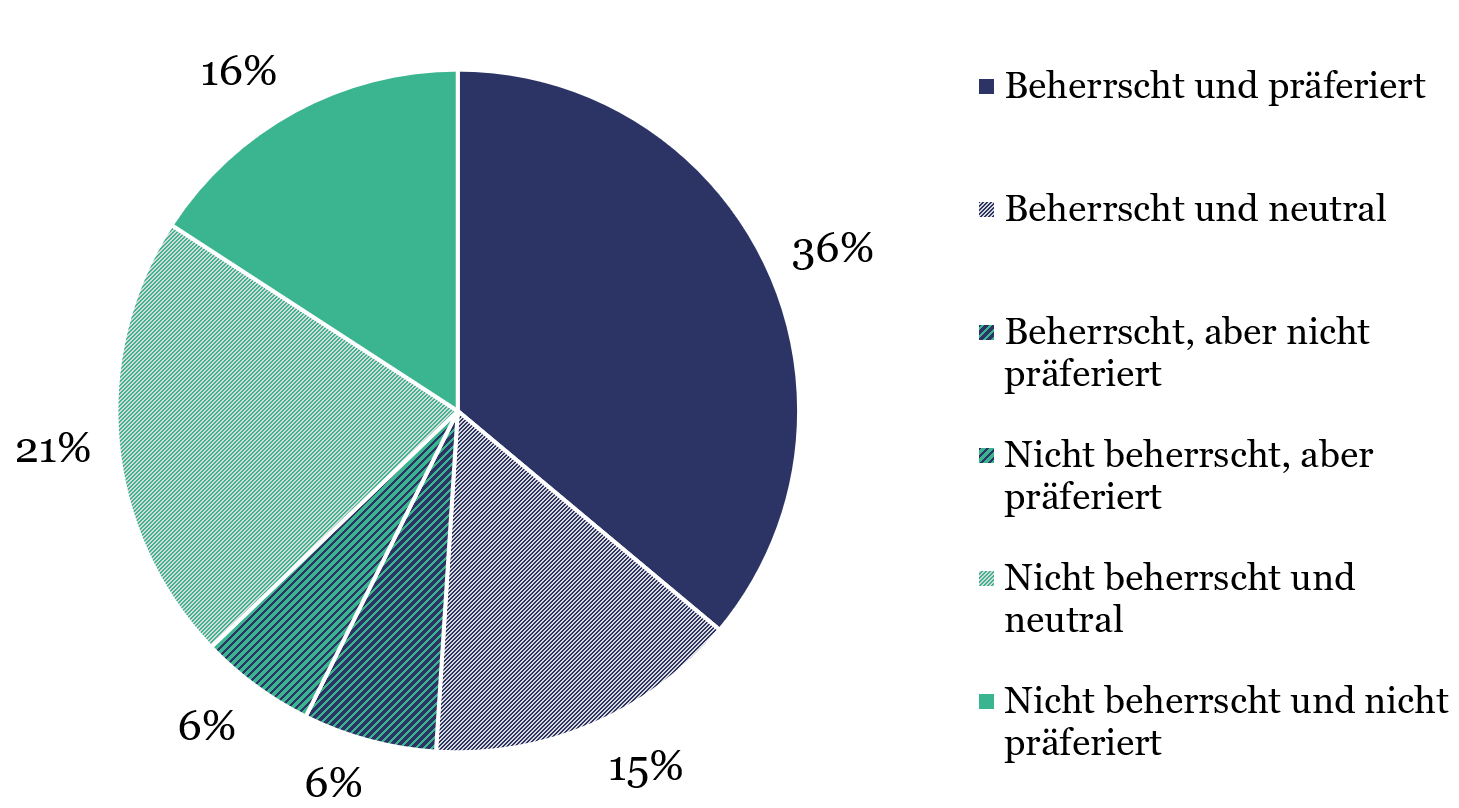
\includegraphics[width=0.9\textwidth]{gfx/verteilung-f-p.png}
	\caption[Durchschnittliche Verteilung der Fähigkeiten und Präferenzen je Mitarbeitenden]{Durchschnittliche Verteilung der Fähigkeiten und Präferenzen je Mitarbeitenden}
	\label{fig:ergebnisse:abb1}
\end{figure}

Aus dem Diagramm geht hervor, dass die Befragten im Durchschnitt mehr Fähigkeiten beherrschen (57 Prozent, blau hinterlegter Bereich), als nicht beherrschen (43 Prozent, orange hinterlegter Bereich).
Mit 36 Prozent beherrscht und präferiert ein Mitarbeitender im Mittel den Großteil der insgesamt angefragten Fähigkeiten (blau markierter Bereich).
Von seinen beherrschten Fähigkeiten will ein Mitarbeitender folglich knapp zwei Drittel zukünftig weiter in Projekten einsetzen (36 von 57 Prozent).
Mit 21 Prozent treten bei einem durchschnittlichen Befragten am zweithäufigsten Fähigkeiten auf, in denen dieser keine Kenntnisse besitzt und indifferent ist, ob er diese Fähigkeiten zukünftig in Projekten anwenden wird, oder nicht (orange hinterlegter Bereich mit grauen Punkten).
Darauf folgen 16 Prozent der angeforderten Fähigkeiten, die ein Mitarbeitender im Mittel nicht beherrscht und auch kein Interesse äußert, diese in zukünftigen anzuwenden (orange markierter Bereich).
Weitere 15 Prozent der Fähigkeiten beherrscht ein durchschnittlicher Mitarbeitender und steht der Option, diese in zukünftigen Projekten einzusetzen, neutral gegenüber (blau hinterlegter Bereich mit grauen Punkten). 
Die übrigen 12 Prozent verteilen sich gleichmäßig auf die Fähigkeiten, die ein Mitarbeitender beherrscht, aber nicht präferiert (blau hinterlegter Bereich mit orangener Schraffierung) und die Fähigkeiten, in denen ein Mitarbeitender keine Kenntnisse besitzt, diese aber präferiert (orange hinterlegter Bereich mit blauer Schraffierung).
Von den beherrschten Fähigkeiten haben Mitarbeitende im Mittel folglich bei circa 10 Prozent kein Interesse, diese beherrschten Fähigkeiten in Projekten (weiter) anzuwenden (6 von 57 Prozent).
Bei den nicht-beherrschten Fähigkeiten beläuft sich der Anteil an Fähigkeiten, die ein Mitarbeitender nicht beherrscht, aber zukünftig gerne in Projekten anwenden würde auf ganze 14 Prozent (6 von 43 Prozent).
% Demnach weist ein Mitarbeitender im Durchschnitt $2$ Fähigkeiten aus, die er nicht beherrscht, aber gerne anwenden würde und 2 Fähigkeiten die er beherrscht, aber kein Interesse hat, diese in Projekten weiter anzuwenden.

Die prozentuale Verteilung der Fähigkeiten und Präferenzen ist in Abbildung \ref{fig:ergebnisse:abb2} in Bezug auf die fünf Beispielprojekte dargestellt.

\begin{figure}
    \centering
	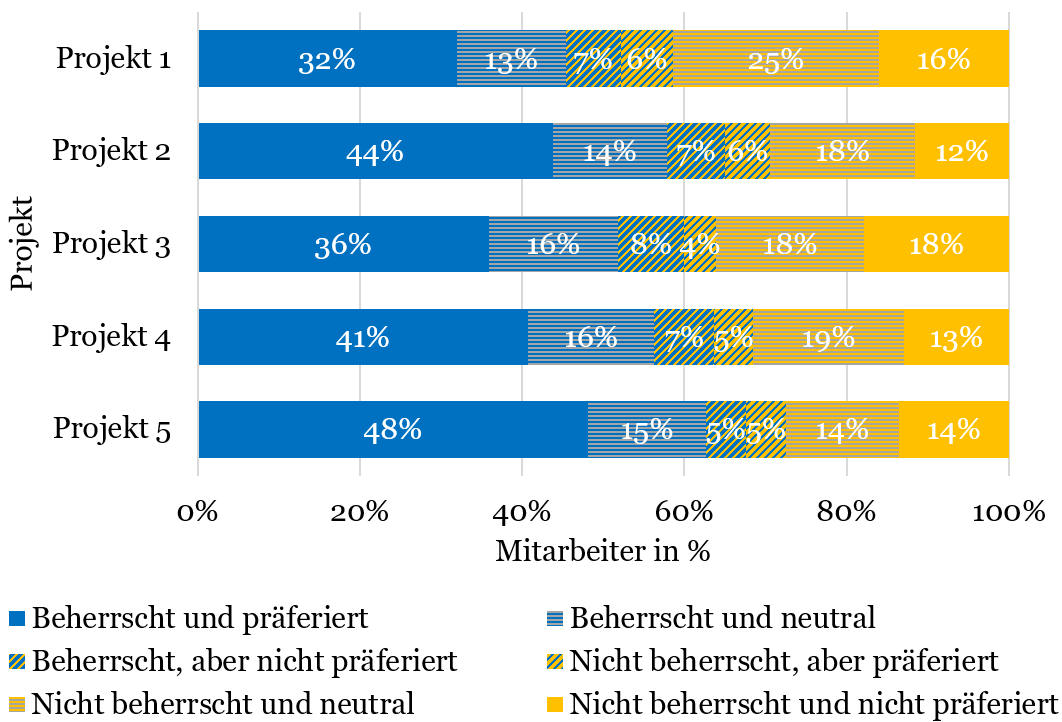
\includegraphics[width=0.9\textwidth]{gfx/verteilung-f-p-nach-projekt.png}
	\caption[Verteilung der Fähigkeiten und Präferenzen nach Projekt]{Verteilung der Fähigkeiten und Präferenzen nach Projekt}
	\label{fig:ergebnisse:abb2}
\end{figure}

Insgesamt wird deutlich, dass sich die Verteilung auf Projektebene nicht maßgeblich von der Ursprungsverteilung unterscheidet.
Jedoch weist sie in einigen Punkten nennenswerte Abweichungen auf.
So geht aus der Abbildung hervor, dass Projekt 5 mit 48 Prozent die meisten Projektpositionen enthält, die Mitarbeitende als beherrscht und präferiert bewertet haben (blau markierter Balken).
Damit liegt die Verteilung der beherrschten und präferierten Fähigkeiten bei Projekt 5 um  12 Prozentpunkte über der Ursprungsverteilung.
Im Gegensatz dazu enthält Projekt 1 mit 32 Prozent die wenigsten Projektpositionen, die von den Befragten als beherrscht und präferiert angegeben wurden.
Diese Verteilung weicht jedoch lediglich um 4 Prozentpunkte von der Ursprungsverteilung ab.
Auch der Anteil der Projektpositionen, die Mitarbeitende nicht beherrschen und auch in zukünftigen Projekten nicht anwenden wollen ist in Projekt 1 mit 16 Prozent im Vergleich zu den anderen Projekten am zweithöchsten (pink markierter Balken).
Lediglich Projekt 3 weist mit 18 Prozent mehr Projektpositionen auf, die Mitarbeitende nicht beherrschen und nicht präferieren.
Der Anteil an Projektpositionen, die Mitarbeitende nicht beherrschen und in denen sie der Option, diese zukünftig in Projekten anzuwenden neutral gegenüberstehen, ist dafür in Projekt 1 mit 25 Prozent am höchsten (pink markierter Balken mit grauer Schraffierung).
Insgesamt weist Projekt 2 den nierdrigsten Anteil an Projektpositionen auf, die Mitarbeitende nicht beherrschen und nicht präferieren.
Dieser liegt mit 12 Prozent 4 Prozentpunkte unter der Ursprungsverteilung.
% Erklärungen für die schwankunen in den Verteilungen in Diskussion anführen -> Erklärung bspw., dass projekte untersch. viele fähigkeiten anfragen und teilweise sehr generisch und am bsp. von projekt 1 sehr spezifisch (bsp. Camunda, welches die fähigkeit ist, die am wenigsten MA beherrschen) (siehe oben auskommentierter text)
% Hier anführen, dass das darauf zurückzuführen sein kann, dass projekt 1 als einziges 12 fähigkeiten verlangt

Bezogen auf die Zufriedenheit gaben die Mitarbeitenden mit 146 von insgesamt 270 Bewertungen (54 Probanden \`{a} je 5 Beispielprojekte) bei mehr als der Hälfte der Optionen an, mit einem Beispielprojekt nicht zufrieden zu sein (Anteile "Gar nicht zufrieden" und "Weniger zufrieden").
Darüber hinaus wurde die Bewertung "Voll und ganz zufrieden" mit 43 Bewertungen am wenigsten von den Befragten angegeben.
Am häufigsten gaben die Mitarbeitenden an mit einem Beispielprojekt gar nicht zufrieden zu sein (83 Bewertungen).
In Abbildung \ref{fig:ergebnisse:abb3} ist die Zufriedenheit der Mitarbeitenden anhand der einzelnen Projekte anteilig abgebildet.
Daraus geht hervor, dass die Mitarbeitenden mit insgesamt 55 Prozent am häufigsten angaben mit Projekt 4 zufrieden zu sein (blauer und grüner Balken).
Im Gegensatz waren die Befragten mit Projekt 3 am wenigsten zufrieden.
Der Anteil der zufriedenen Mitarbeitenden lag hier bei 31 Prozent.
Verglichen mit der Verteilung der Fähigkeiten und Präferenzen in Abbildung \ref{fig:ergebnisse:abb2} fällt auf, dass bei Projekt 3 auch der Anteil der Fähigkeiten, die von den Mitarbeitenden nicht präferiert wurden mit 26 Prozent am höchsten ausfiel (blau hinterlegter Balken mit pinker Schraffur und pink markierter Balken).
% HIER WEITERMACHEN

\begin{figure}
    \centering
	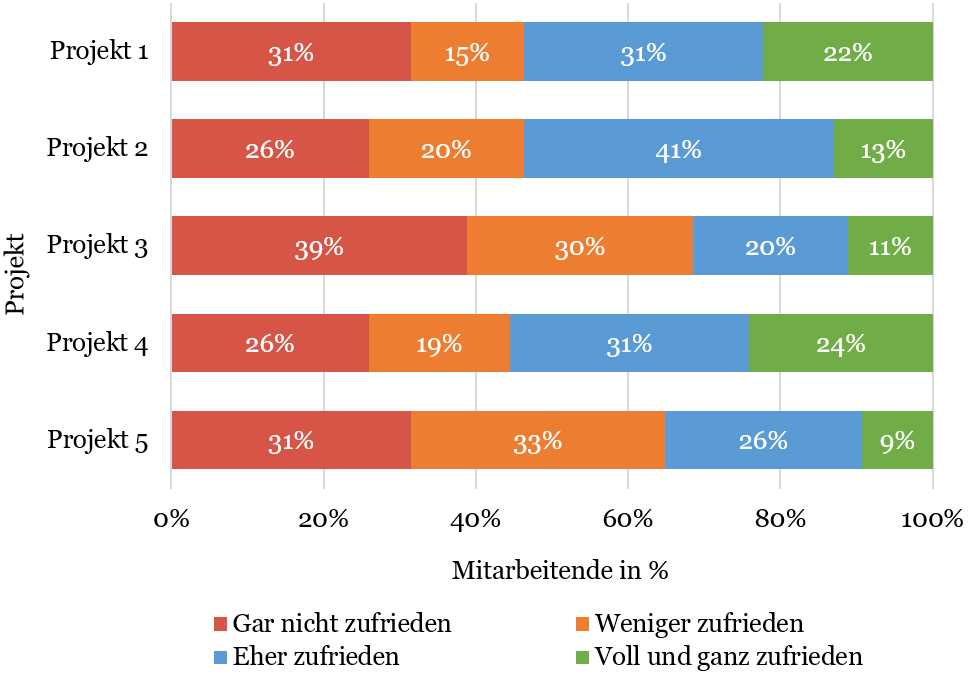
\includegraphics[width=0.9\textwidth]{gfx/verteilung-z-nach-projekt.png}
	\caption[Zufriedenheit der Mitarbeitenden nach Projekt]{Zufriedenheit der Mitarbeitenden nach Projekt}
	\label{fig:ergebnisse:abb3}
\end{figure}

Dann ansehen wie Zufrieden die MA mit projekten sind
und wie die ma fähigkeiten je projekt besitzen

\section{Überblick Befragung der Manager}

\section{Evaluation des Algorithmus}

\shorthandon{"}